

\begin{frame}{Componentes CheckBox e ImageView en Android}

\textbf{CheckBox: ¿Para qué sirve?}
\begin{itemize}
    \item Permite al usuario seleccionar una o múltiples opciones de una lista.
    \item Cada opción es independiente (no excluyente).
    \item Es útil en formularios, configuraciones o encuestas.
\end{itemize}

\vspace{0.4cm}

\textbf{Características del CheckBox:}
\begin{itemize}
    \item Puede estar en estado seleccionado o no seleccionado.
    \item Permite manejar eventos de cambio (OnCheckedChangeListener).
\end{itemize}

\vspace{0.4cm}

\textbf{ImageView: ¿Para qué sirve?}
\begin{itemize}
    \item Se utiliza para mostrar imágenes en la interfaz de usuario.
    \item Soporta recursos locales (drawable) o imágenes desde URL.
\end{itemize}

\vspace{0.4cm}

\textbf{Características del ImageView:}
\begin{itemize}
    \item Permite escalar, ajustar y posicionar imágenes.
    \item Compatible con diferentes formatos (PNG, JPG, SVG - mediante librerías).
\end{itemize}


\end{frame}


\begin{frame}[fragile]
\frametitle{Demo 04: Agregar un CheckBox y un ImageView}
\begin{columns}
\column{0.80\linewidth}
Del Repositorio Github:
\begin{itemize}
\item Copiar el archivo MainActivity\_Demo04.java (dentro del Folder códigosJAVA) al mismo directorio donde esta el MainActivity.java
\item Copiar el archivo activity\_main\_demo04.xml (dentro del Folder Carpeta\_layout) al mismo directorio donde esta el activity\_main.xml
\item Copiar el archivo \textit{upv.png} dentro de la folder \textit{Carpeta\_drawable} en el directorio \textit{res/drawable} del proyecto de AS.


\item Modificar en el archivo AndroidManifest.xml la cadena \textit{.MainActivity\_Demo03} por \textit{.MainActivity\_Demo04}
\end{itemize}

\begin{block}{Demo \#04}
Una App con in Checkbox y un ImageView. Al modificar el estado del CheckBox, el texto de un Textview cambia. Al presionar el primer boton, un Toast muestra el estado del Checkbox.  
\end{block}


\column{0.20\linewidth}

\begin{center}
 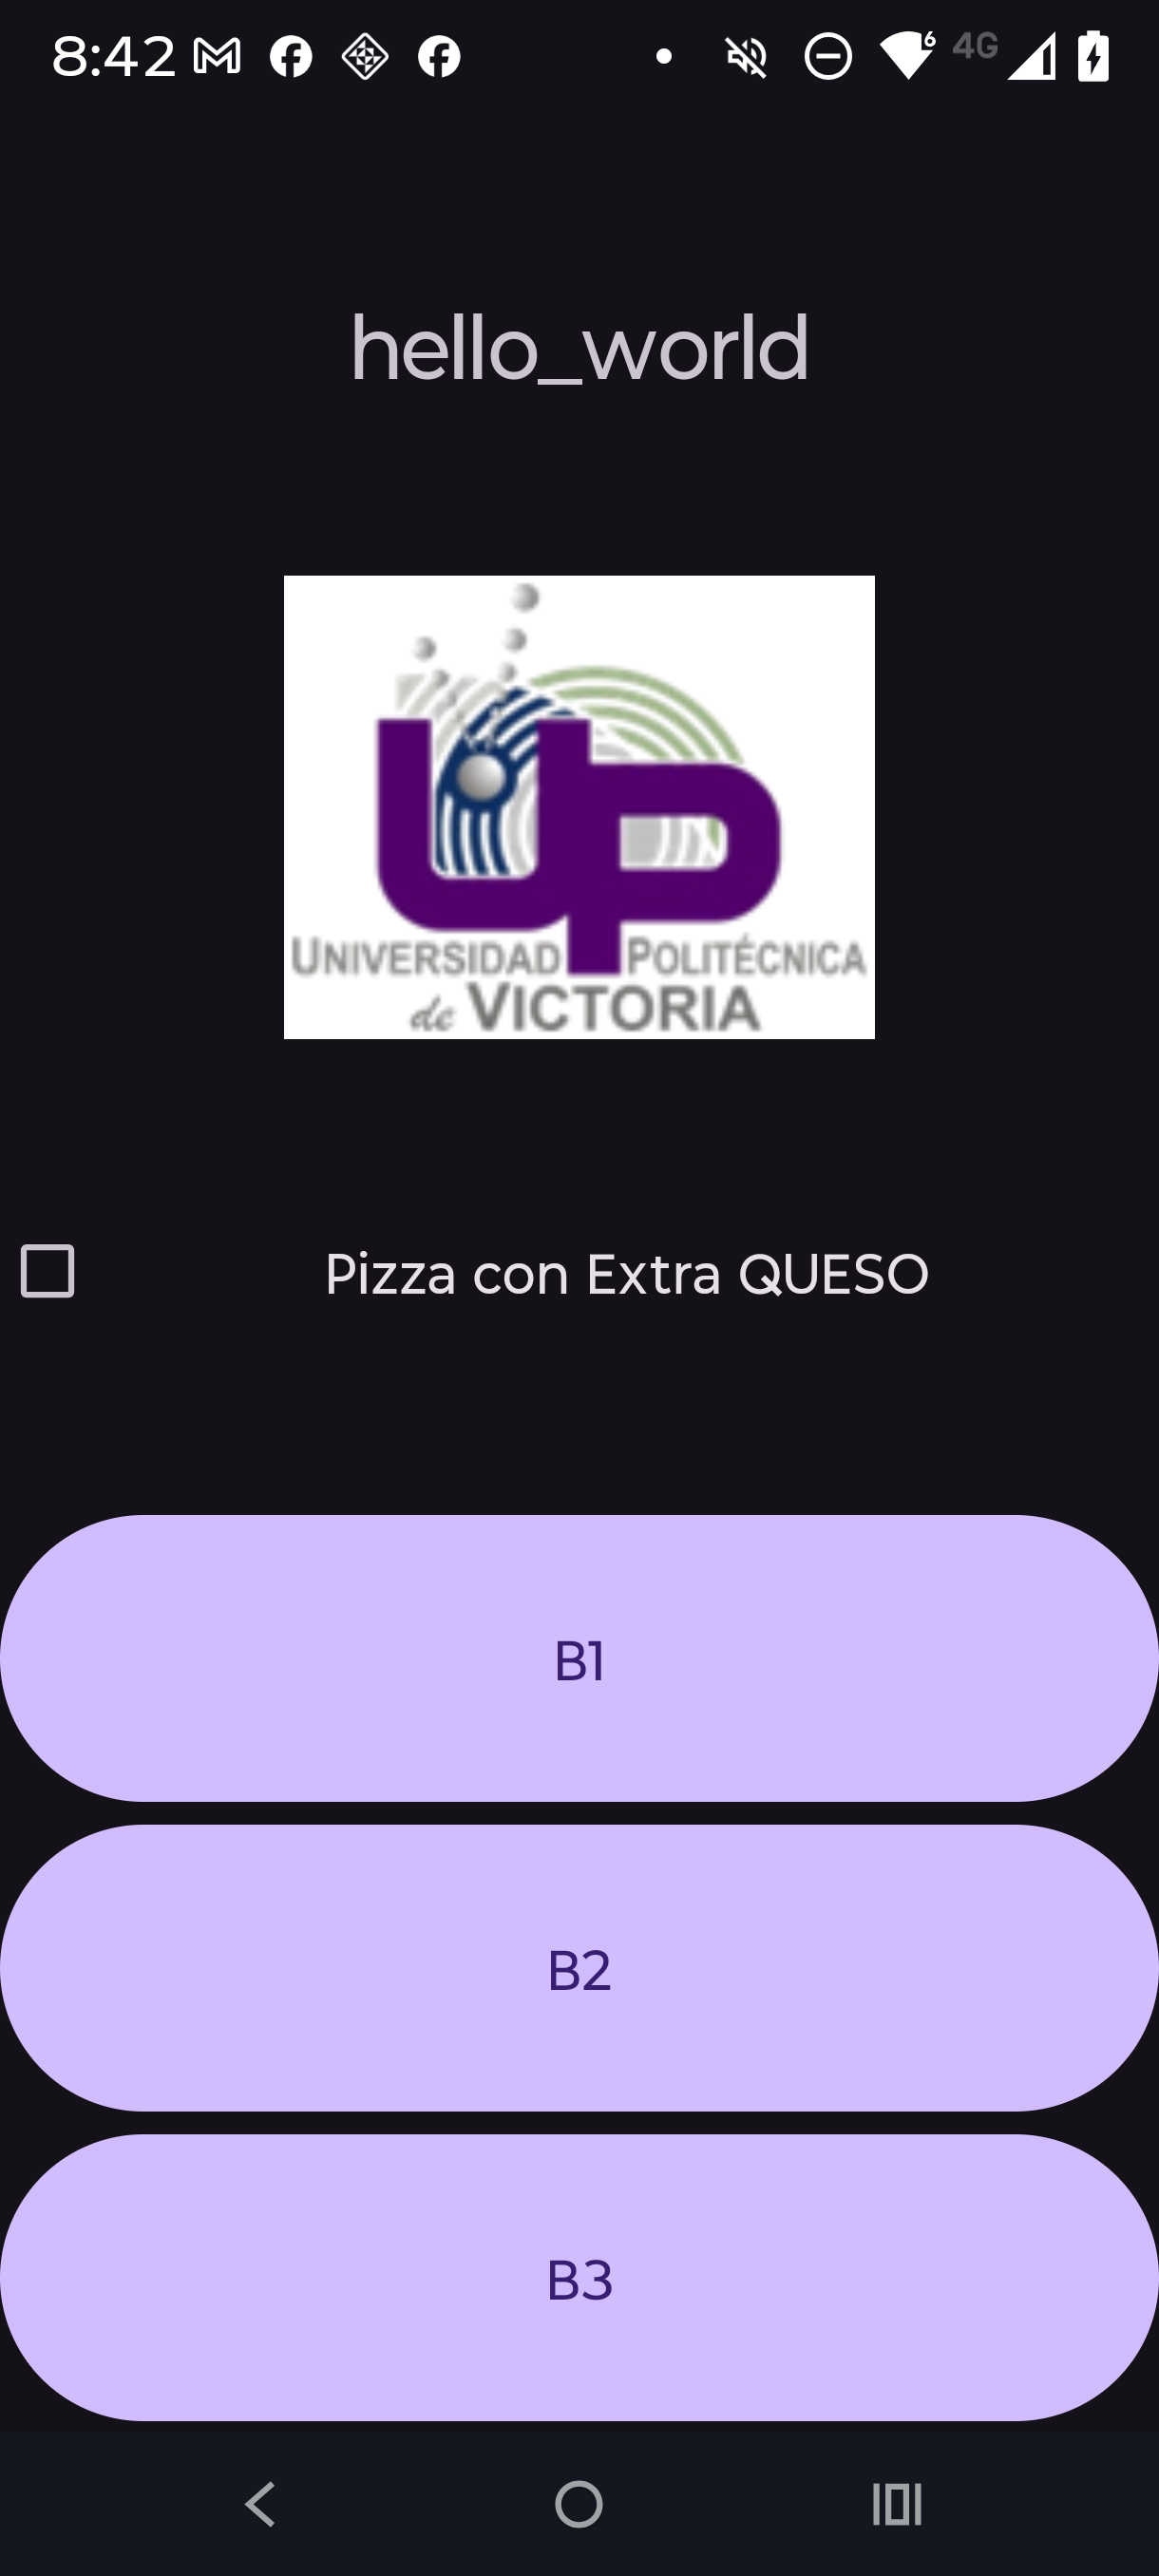
\includegraphics[width=0.98\textwidth]{02_TallerCBTis/figs/Demo04}
\end{center}

\end{columns}

\end{frame}


